
%(BEGIN_QUESTION)
% Copyright 2011, Tony R. Kuphaldt, released under the Creative Commons Attribution License (v 1.0)
% This means you may do almost anything with this work of mine, so long as you give me proper credit

Read and outline the ``Selector Controls'' subsection of the ``Limit, Selector, and Override Controls'' section of the ``Basic Process Control Strategies'' chapter in your {\it Lessons In Industrial Instrumentation} textbook.  Note the page numbers where important illustrations, photographs, equations, tables, and other relevant details are found.  Prepare to thoughtfully discuss with your instructor and classmates the concepts and examples explored in this reading.

\underbar{file i02469}
%(END_QUESTION)





%(BEGIN_ANSWER)


%(END_ANSWER)





%(BEGIN_NOTES)

A ``selector'' control system is one where multiple measurement or setpoint signals are selected to go into a single controller.

Selection function blocks may be applied to redundant transmitters, to provide ``greatest,'' ``least,'' or ``median'' signal selection to obtain the most reliable measurement for some critical application.  Median (middle-value) signal selection may be done by selecting the lowest value of the highest values from pairs of inputs, or by selecting the highest value of the lowest values from pairs of inputs.

\vskip 10pt

CS function block (FOUNDATION Fieldbus) used to select controller outputs (for override strategies).  ISEL function block (FOUNDATION Fieldbus) used to select measurement or setpoint signals (for selector strategies).

When installing redundant transmitters, never install just two.  Always install {\it three} at minimum!

\vskip 10pt

Air:fuel ratio in the first control system shown tends to vary as the firing rate rapidly changes.  Since fuel is wild and air is captive, air flow tends to lag behind fuel flow.  This leads to rich burn conditions as firing rate increases, and to lean burn conditions when firing rate decreases.  Rich burning may lead to an explosion, while lean burning may lead to flame-out.  Cross-limiting is where high- and low-select functions are installed in such a way that the air flow setpoint is always the {\it greatest} and fuel flow setpoint is always the {\it least}, selected between the firing rate signal versus the other flow transmitter.

{\it Multiplier} and {\it divider} functions may be installed in a cross-limited ratio control system to allow a single air:fuel ratio command signal to influence both controller setpoints.









\filbreak


\vskip 20pt \vbox{\hrule \hbox{\strut \vrule{} {\bf Suggestions for Socratic discussion} \vrule} \hrule}

\begin{itemize}
\item{} Explain the purpose of the three-temperature transmitter system shown at the beginning of this section.
\item{} {\bf Demonstrate how either of the median-select strategies works, by plugging sample values into the three inputs and proving that the output is always the middle of the three sample values.}
\item{} How does the ISEL function block calculate the median value for {\it four} good inputs?
\item{} Explain why it is always preferable to use {\it three} transmitters instead of {\it two} when building redundant systems.
\item{} Explain why the CS function block provides {\tt BKCAL\_OUT} signal outputs but the ISEL function block does not.
\item{} Explain why the simple (non-limited) air/fuel ratio control system presents a hazard when the firing command signal steps.
\item{} Identify the consequences of the air flow transmitter in the simple (non-limited) air/fuel ration system failing with a low signal
\item{} Identify the consequences of the air flow transmitter in the simple (non-limited) air/fuel ration system failing with a high signal
\item{} Identify the consequences of the fuel flow transmitter in the simple (non-limited) air/fuel ration system failing with a low signal
\item{} Identify the consequences of the fuel flow transmitter in the simple (non-limited) air/fuel ration system failing with a high signal
\item{} {\bf Explain how the cross-limiting control strategy works to minimize hazards in a large burner system.}
\item{} Identify the consequences of the air flow transmitter in the cross-limited air/fuel ration system failing with a low signal
\item{} Identify the consequences of the air flow transmitter in the cross-limited air/fuel ration system failing with a high signal
\item{} Identify the consequences of the fuel flow transmitter in the cross-limited air/fuel ration system failing with a low signal
\item{} Identify the consequences of the fuel flow transmitter in the cross-limited air/fuel ration system failing with a high signal
\end{itemize}










\vfil \eject

\noindent
{\bf Prep Quiz:}

Determine the value of this selector function's output signal, in percent:

$$\includegraphics[width=15.5cm]{i01782x03.eps}$$


\vfil \eject

\noindent
{\bf Prep Quiz:}

Determine the value of this selector function's output signal, in percent:

$$\includegraphics[width=15.5cm]{i01782x04.eps}$$

%INDEX% Reading assignment: Lessons In Industrial Instrumentation, basic control strategies (selector controls)

%(END_NOTES)


